\subsection{Dataset}
\label{subsec:dataset}

In this section, we describe the selection criteria that guided our choice of the Mushroom and Hepatitis datasets and analyze their respective characteristics.

\subsubsection{Dataset Selection}
In this project, we aimed to select two datasets that offer substantial variability across different aspects to evaluate the performance of Support Vector Machine (SVM) and k-Nearest Neighbors (KNN) algorithms.
The criteria for dataset selection were centered around having one dataset that is small and another that is large, allowing us to analyze both the efficiency and effectiveness of these models across differing dataset sizes.
A smaller dataset, enables rapid experimentation and comparison of SVM and KNN performance.
Meanwhile, a larger dataset, provides an excellent opportunity to evaluate the benefits of reduction methods in KNN, especially regarding storage efficiency and reduced running time.

Moreover, we wanted to assess the models' ability to handle datasets with different types of attributes.
For this purpose, we wanted to select one dataset with primarily nominal attributes and another with numerical features.
This allows us to evaluate how well each algorithm handles the representation and processing of different data types.
Additionally, class distribution was a critical factor in our selection. By choosing one dataset with a balanced distribution and another with a notable class imbalance, we aim to observe how SVM and KNN, particularly with reduction, perform in scenarios where the data is skewed.
Lastly, we prioritized finding datasets with varying levels of missing data to examine how effectively the algorithms manage incomplete information.

Based on these criteria, we selected the Hepatitis and Mushroom datasets, as they provide the most distinct and complementary combination for our evaluation.

\subsubsection{Dataset Characteristics}

\begin{figure}
    \centering
    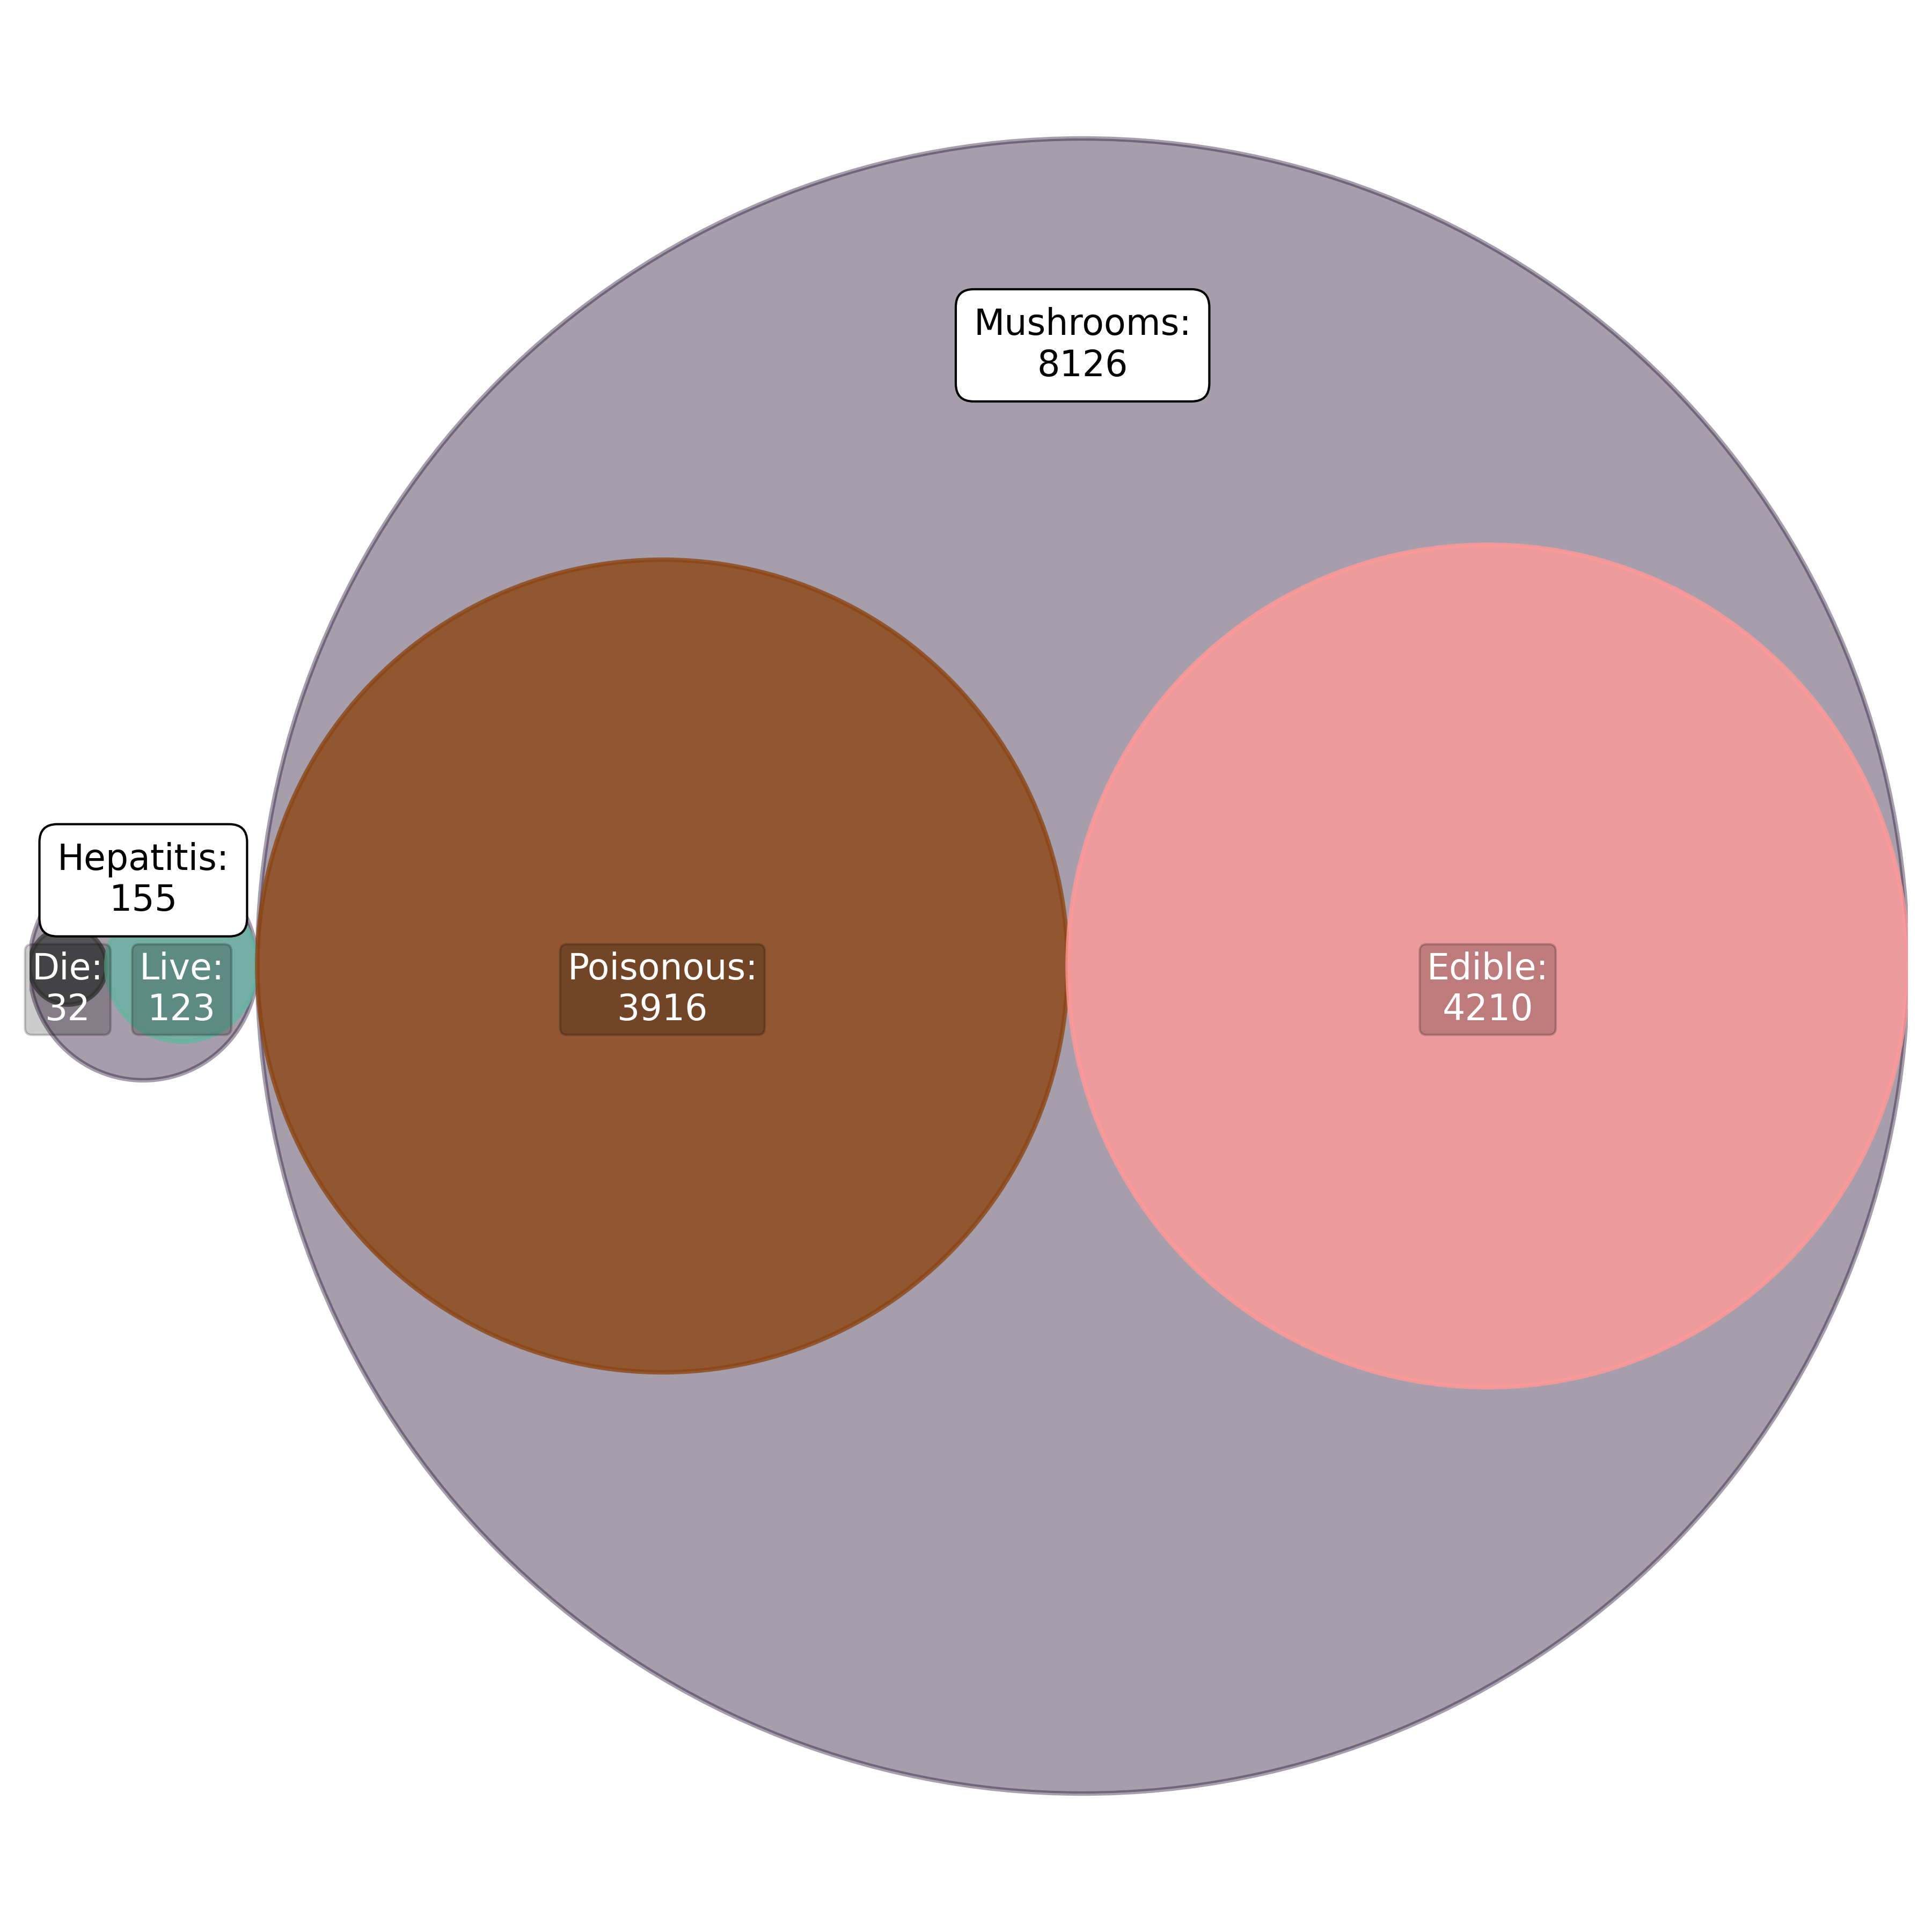
\includegraphics[width=0.5\textwidth]{figures/dataset-partitions.png}
    \caption{Dataset partitions}
    \label{fig:dataset-partitions}
\end{figure}

The Mushroom dataset, with 8,124 instances, is much larger (see \autoref{fig:dataset-partitions}) than the Hepatitis dataset's 155 instances, making it ideal for examining the computational benefits of reduction techniques.
The Mushroom dataset focuses on predicting whether a mushroom is poisonous or edible based on 22 nominal attributes, such as cap shape and color, whereas the Hepatitis dataset aims to predict whether a hepatitis patient will live or die, using a mix of both nominal and numeric features like age and liver size.
This allows for a comparison of model handling for fully categorical data versus mixed data types.

\begin{figure}
    \centering
    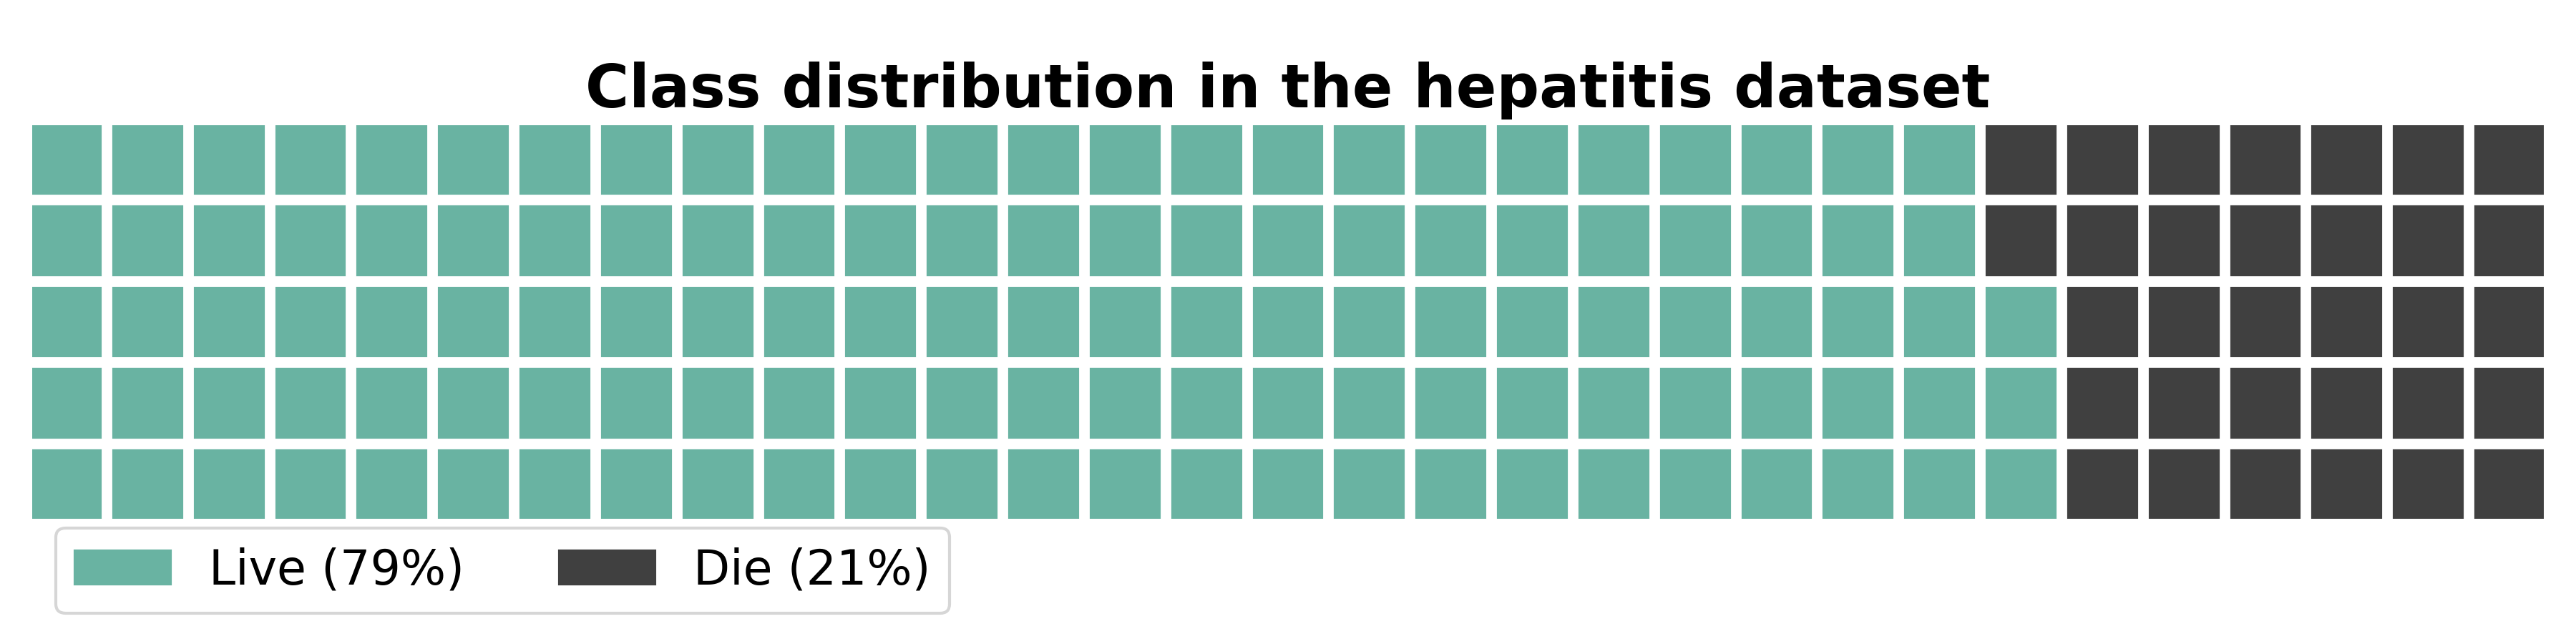
\includegraphics[width=0.45\textwidth]{figures/hepatitis-class-distribution.png}
    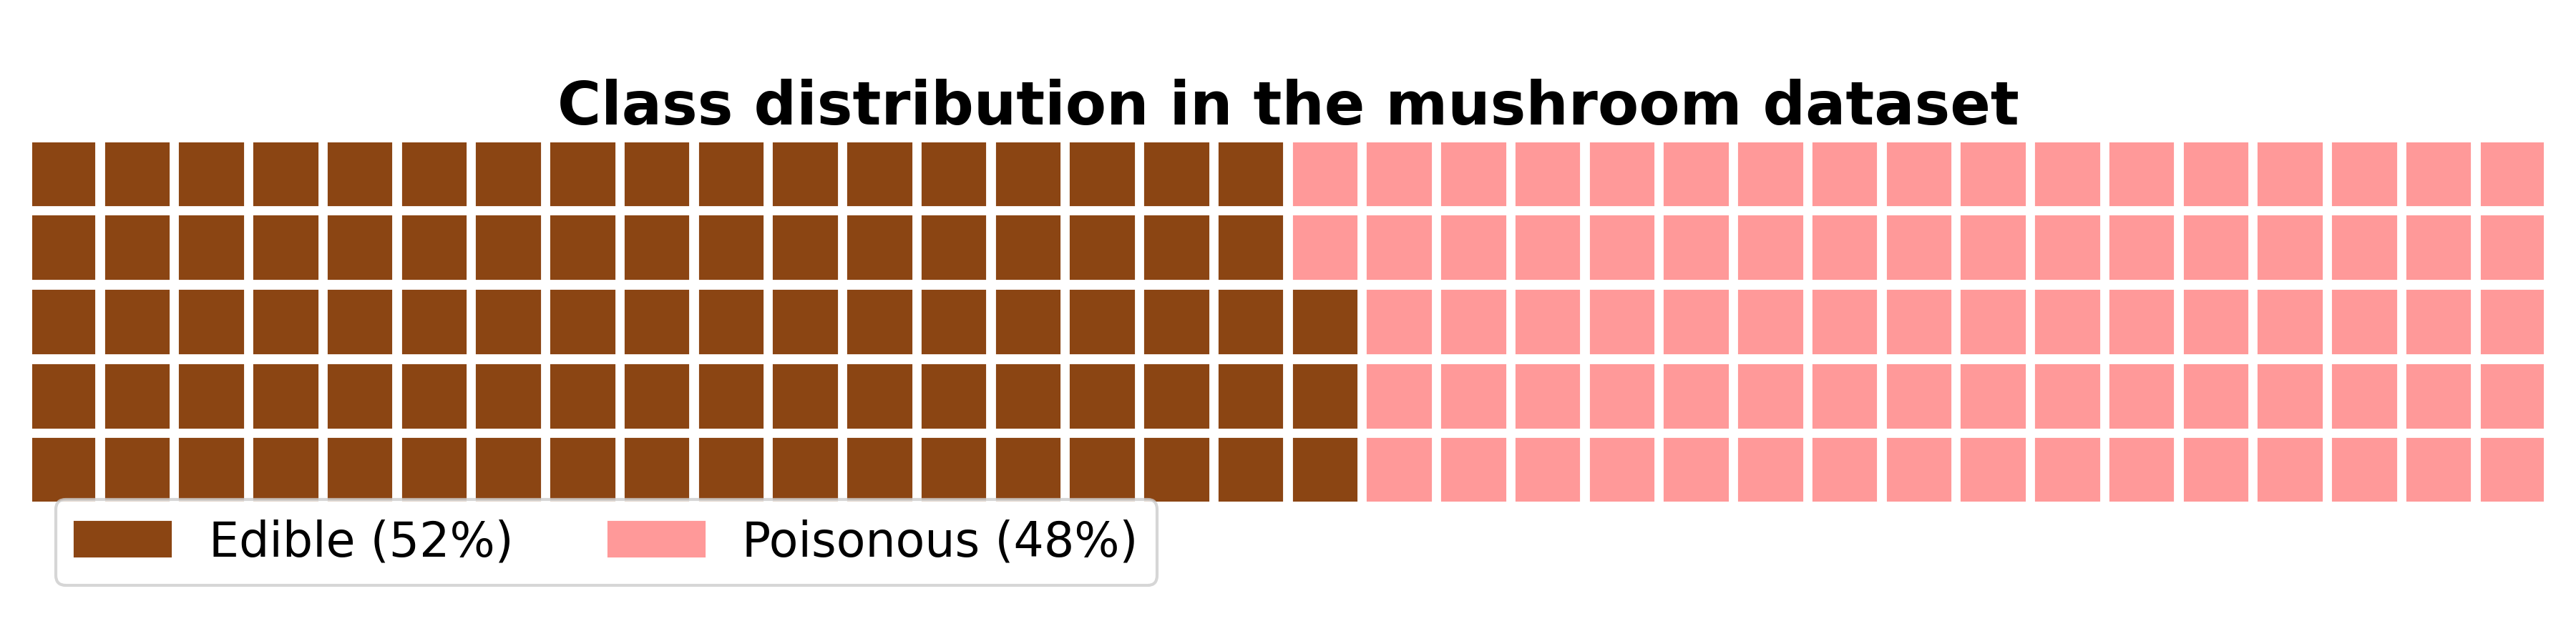
\includegraphics[width=0.45\textwidth]{figures/mushroom-class-distribution.png}
    \caption{Class distributions}
    \label{fig:class-distributions}
\end{figure}

Class distribution is another key distinction.
The Mushroom dataset is nearly balanced, with only a 1.8\% class deviation, while the Hepatitis dataset has a 29.35\% class deviation, with 79.35\% of instances in the majority class (see \autoref{fig:class-distributions}), making it ideal for testing each model's robustness to imbalanced data.
Missing data is also more prevalent in the Mushroom dataset (48.2\%) compared to Hepatitis (20.01\%), providing insights into each model’s ability to handle incomplete data.